Graph theory is used widely and it is possible and desirable to implement graph traversals in parallel since graphs can be quite large.
This section does not describe graph theory in depth, but explains some basic notions of graphs and then describes how graph traversals can be implemented in parallel.
There are two types of graphs: undirected and directed graphs.
This section only considers undirected graphs.
An undirected graph \textit{G} is represented as a pair \textit{(V, E)}, where
\begin{itemizeSmall}
	\item[\textbf{V}:] $V\notin \{\}$ and is called the set of vertices. A vertex can also be denoted as a "node".
	\item[\textbf{E}:] set of unordered pairs of vertices and is called the set of edges.
	\item[\textbf{(u, v)}] is an edge which has two endpoints \textit{u} and \textit{v} where both are vertices.
\end{itemizeSmall}

\noindent A graph can be traversed and this means that each node of the graph is visited.
There are two types of graph traversals: breadth-first search, \textbf{BFS}, and depth-first search, \textbf{DFS}.
A breadth-first search traversal begins at a particular node and visits all neighboring nodes that are one hop away and labels them as they are visited. 
Then all nodes which have been visited one hop away from the starting point are now visiting all their one-hop-away neighbors. 
This is done iteratively until all nodes have been labeled and thus visited.
An example is seen in \autoref{fig:bfs}.
A "frontier" forms a boundary between all nodes that already has been visited.
This means that the frontier will be expanded during the traversal of a given graph.

A depth-first search traversal begins at a particular node and picks a neighboring node which has not been visited yet. 
This node is then labeled as visited and yet another depth-first traversal is done from this node. 
If a node does not have an unvisited neighbor then it goes to a previously labeled node and picks an unlabeled neighboring node. 
This process is done iteratively until all nodes have been labeled as visited.
The process of a depth first traversal is shown in \autoref{fig:dfs}.
\begin{figure}[ht]
	\begin{subfigure}{0.5\textwidth}
		\begin{center}
			\fbox{
				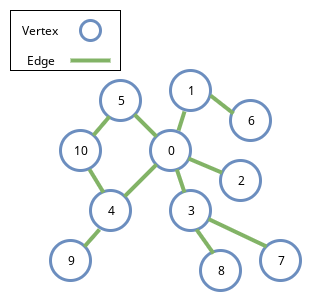
\includegraphics[width=0.5\textwidth]{figs/apps/bfs.png}
			}
		\end{center}
		\caption{Breadth-first traversal example}
		\label{fig:bfs}
	\end{subfigure}%
	\begin{subfigure}{0.5\textwidth}
		\begin{center}
			\fbox{
				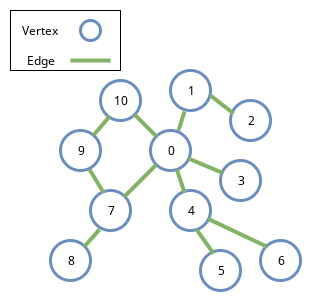
\includegraphics[width=0.5\textwidth]{figs/apps/dfs.png}
			}
		\end{center}
		\caption{Depth-first traversal example}
		\label{fig:dfs}
	\end{subfigure}
	\caption{Graph traversal examples}
\end{figure}

\noindent In general the \textit{DFS} is more memory efficient since it requires less state, but \textit{BFS} exposes more parallelism during the iterative traversal stages.
For this reason only \textit{BFS} is considered in parallel.

The hop distance from a \textit{root} node to the furthest away node is denoted as the depth of graph.
\begin{figure}[ht]
	\begin{subfigure}{0.5\textwidth}
		\begin{center}
			\fbox{
				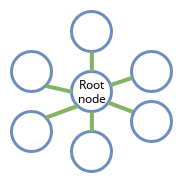
\includegraphics[width=0.3\textwidth]{figs/apps/stargraph.png}
			}
		\end{center}
		\caption{Star shaped graph}
		\label{fig:stargraph}
	\end{subfigure}%
	\begin{subfigure}{0.5\textwidth}
		\begin{center}
			\fbox{
				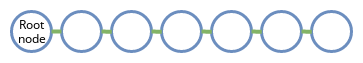
\includegraphics[width=0.7\textwidth]{figs/apps/chaingraph.png}
			}
		\end{center}
		\caption{Chain shaped graph}
		\label{fig:chaingraph}
	\end{subfigure}
	\caption{Types of graphs}
\end{figure}
A graph with \textit{N} nodes can have a minimum possible graph depth of one.
In this case it will be a star shaped graph as depicted in fig \autoref{fig:stargraph}.
This kind of graph exploits a lot of parallelism since each "branch" in the graph can be processed independently.
Conversely, a graph can have a maximum depth of $N-1$.
If this is the case the graph is formed as a linear chained shape as seen in \autoref{fig:chaingraph}.
A linear chained graph is hard to parallelize since it would take \textit{n} steps to traverse the graph.
This also gives the worst case step complexity as described in \autoref{sec-step-comp}.
\\\\
Now a fundamental understanding of graphs and graph traversals has been established. This brings us to how a \textbf{BFS} traversal can be implemented in a parallel algorithm.
The high level algorithm of a BFS can be characterized  as:
\begin{center}
	\fbox{
		\begin{tabular}{p{40pt} p{220pt}}
			\textbf{Step 1} & Parallelize over list of edges \\
			\textbf{Step 2} & Iterate \textit{n} times, where \textit{n} is the maximum depth of the graph \\
			\textbf{Step 3} & For each iteration, if a vertex has depth \textit{d} and another vertex has not been visited then the unvisited vertex gets $d+1$
		\end{tabular}
	}
	\captionof{table}{Steps to BFS traversal}
	\label{alg-bfs}
\end{center}
For example if we have a undirected graph defined as
\begin{align}
	G_{example} &= (V, E) \text{, where}   \label{eq:gex}\\
			  V &= \{0, 1, 2, 3, 4, 5, 6\} \\
			  E &= \{(0, 1), (1, 2), (2, 3), (3, 4), (5, 2), (6, 5) \}
\end{align}
\begin{wrapfigure}{r}{0.21\textwidth}
	\centering
	\fbox{
		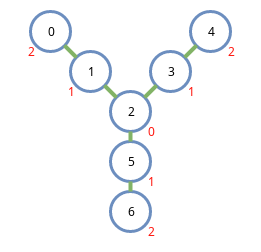
\includegraphics[width=0.2\textwidth]{figs/apps/bfsex.png}
	}
	\caption{BFS parallel example} 
	\label{fig:bfsex}
\end{wrapfigure}
If the BFS is started at node two then notice that the maximum depth is two, since the furthest away neighbors are two hops away.
Thus the expected number of iterations in the BFS traversal in this case is two.
The first step is to look at all edges in parallel.
Node two has a $d=0$ and in the list of edges the node two appears in three pairs namely the pairs (1, 2), (2, 3) and (5, 2).
This means that in the first iteration nodes 1, 3 and 5 will be assigned $d = d_{2} + 1$ and marked as visited.
In the second iteration we look at whether there are more nodes that have not been visited.
This is the case for nodes 0, 4 and 6.
The nodes appear in pairs (0, 1), (3, 4) and (6, 5).
In this iteration nodes 0, 4 and 6 will be assigned $d = d_{1, 3, 5} + 1$ and marked as visited.
Each iteration in this case of BFS can be computed by running 6 threads in parallel.
A visualization of BFS traversal of \autoref{eq:gex} is shown in \autoref{fig:bfsex} where the red numbers indicate in which order they have been visited in parallel.

Concerning work complexity of BFS on a graph the maximum number of iterations there can be for the worst case chained linear graph, depicted in \autoref{fig:chaingraph}, is $card(V)$ and the number of computations that has to be made is $card(E)$.
Thus the total running time becomes $O(V\cdot E)$.
Mostly, interesting graphs have more edges than vertices and thus at worst the running time can be $O(V^2)$ which is a big drawback of this kind of implementation of BFS in parallel.